\section{Kompressionsstandard BrotliG}
\label{sec:brotlig}
asdfasdf


\subsection{LZ77}
\label{subsubsec:lz77}
Der LZ77 (\textit{Lempel-Ziv77}) Algorithmus gehört zu der Gruppe der Phrasenkodierung und ist ein verlustfreier, auf einem Wörterbuch basierender Algorithmus.
Der Algorithmus komprimiert sequentielle Zeichenketten.
Dabei kann dieser auf jeder Art von Daten, egal wie der Inhalt und die Größe aussieht, angewendet werden.
Ob es sich lohnt, diesen anzuwenden, ist jedoch von den Daten abhängig.
Beispielsweise sind Bilder ein schlechter Anwendungsfall, da sich die Informationen nur im Ausnahmefall wiederholen, und es deutlich bessere Kompressionsalgorithmen zur Komprimierung dieser gibt.
Das Ziel des LZ77 Algorithmus ist lediglich, redundante Informationen zusammenzufassen. \newline

Bevor der Algorithmus beschrieben wird, werden die benötigten Elemente definiert:

\begin{enumerate}
\item{Eingabestrom:} Die zu kodierenden Daten
\item{Symbol:} Ein willkürlich gewähltes Element des Eingabestroms
\item{Datenfenster:} Alle Symbole vom Start des Eingabestroms bis zum aktuell betrachteten Symbol
\item{Vorschaufenster:} Ein Buffer fester Größe der Symbole vom aktuell betrachteten Symbol bis zum Ende des Buffers enthält
\item{Schiebefenster:} Daten- und Vorschaufenster
\item{Codewort:} Ein Codewort bestehend aus dem Offset, der Lauflänge und des zu kodierenden Symbols
\end{enumerate}

Der Ablauf des Algorithmus besteht aus folgenden Schritten:

Zu Beginn des Algorithmus wird das Datenfenster auf den Start des Eingabestroms gesetzt.
Dieses Fenster ist zunächst leer.
Das Vorschaufenster wird vom Start des Eingabestroms mit Symbolen gefüllt, bis dieses voll ist.
Zunächst wird das erste Symbol kodiert.
Dafür verwendet der LZ77 Algorithmus ein Tupel in der Form von (\textit{Position}, \textit{Lauflänge}) und abschließend das zu kodierende Symbol.
Dem Wörterbuch noch nicht bekannt Symbole werden neue Symbole mit (0, 0)Symbol hinzugefügt.
Nach jedem Schritt wird das Schiebefenster um die Lauflänge der kodierten Symbole im Eingabestrom verschoben
\cite{lz2023}.

\subsubsection{Kodierung eines Codewortes}
\label{subsubsec:kodierung_codewort}
Zur Veranschaulichung wird das Codewort \glqq laufenraufen\grqq\ mit dem LZ77 Algorithmus kodiert und anschließend wieder dekodiert.
Daten- und Vorschaufenster haben in diesem Beispiel eine Kapazität von jeweils sechs Symbolen.
\begin{table}[]
\centering
\begin{tabular}{|l|l|l|l|}
\hline
\textbf{Datenfenster} & \textbf{Vorschaufenster} & \textbf{restliches Codewort} & \textbf{Kodierung} \\ \hline
                      & laufen                   & raufen                       & (0, 0)l            \\ \hline
l                     & aufenr                   & aufen                        & (0, 0)a            \\ \hline
la                    & ufenra                   & ufen                         & (0, 0)u            \\ \hline
lau                   & fenrau                   & fen                          & (0, 0)f            \\ \hline
lauf                  & enrauf                   & en                           & (0, 0)e            \\ \hline
laufe                 & nraufe                   & n                            & (0, 0)n            \\ \hline
laufen                & raufen                   &                              & (0, 0)r            \\ \hline
aufenr                & aufen                    &                              & (6, 4)n            \\ \hline
\end{tabular}
\end{table}

Eine Besonderheit die zunächst nicht intuitiv ist, ist die Konstruktion des letzten Codewortes in diesem Beispiel.
Die Symbolsequenz \glqq aufen\grqq\ mit der Kodierung \textit{6, 4)n} könnte auch mit einem Offset von fünf kodiert werden.
Im Normalfall würde die Symbolsequenz auch so kodiert werden.
Da jedoch das Symbol \glqq n\grqq\ das letzte Symbol des zu kodierenden Worts ist, und es so kein weiteres, zu kodierendes Symbol gibt, muss die Länge um eins reduziert werden, und das letzte Symbol kodiert werden. \newline

Aus dem Beispiel geht hervor, das die Auswahl der Buffergröße gut gewählt werden muss, damit der Algorithmus effektiv verwendet werden kann.
Wäre in dem Beispiel das Datenfenster lediglich Platz für vier statt fünf Symbole, hätte die Symbolsequenz \glqq aufe\grqq nicht als ganzes kodiert werden können.
Die weiteren Iterationen der Lempel-Ziv Algorithmen haben statt einem lokalen Wörterbuch (Datenfenster) ein globales Wörterbuch verwendet.
Durch die große Anzahl an Vergleichen erreicht der LZ77 Algorithmus ein besseres Kompressionsverhältnis als der LZ78 Algorithmus, benötigt für die Kompression jedoch länger.
Wie lange das Komprimieren der Daten dauert ist jedoch nicht wichtig für diese Arbeit.
Der interessante Punkt ist die Dekompressionsgeschwindigkeit.
Der LZ77 Algorithmus ist bedeutend schneller bei der Dekomprimierung als bei der Komprimierung \cite{Choudhary2015}.

\subsubsection{Dekodierung eines Codeworts}
\label{subsubsec:dekodierung_codewort}
In diesem Abschnitt soll aus der Kodierung wieder das zuvor festgelegte Codewort generiert werden.
\begin{table}[]
\centering
\begin{tabular}{|l|l|l|}
\hline
\textbf{Kodierung} & \textbf{Datenfenster}         & \textbf{Codewort} \\ \hline
(0, 0)l            &                               & l                 \\ \hline
(0, 0)a            & l                             & la                \\ \hline
(0, 0)u            & la                            & lau               \\ \hline
(0, 0)f            & lau                           & lauf              \\ \hline
(0, 0)e            & lauf                          & laufe             \\ \hline
(0, 0)n            & laufe                         & laufen            \\ \hline
(0, 0)r            & laufen                        & laufenr           \\ \hline
{\color[HTML]{009901}(6, 4)n}            & {\color[HTML]{009901} aufe}nr & laufenr{\color[HTML]{009901} aufen}      \\ \hline
\end{tabular}
\end{table}

Wie zu sehen ist, ist der LZ77 Algorithmus sowohl leicht verständlich als auch effektiv, wodurch er seinen Nutzen in vielen Anwendungen findet.
Seine Weiterentwicklungen nennen sich LZ78 und LZW, die zwar dem LZ77 Algorithmus technisch überlegen sind, aufgrund von Patenten jedoch nicht so eine große Rolle spielen wie die erste Iteration von Lempel und Ziv.
In Kombination mit anderen Techniken wie der Huffman Codierung bildet der LZ77-Algorithmus jedoch die Grundlage vieler leistungsstarker Kompressionsstandards, die heute in vielen Applikationen zu finden sind [QUELLE!!!]. \newline


\subsection{Huffman Codierung}
\label{subsec:huffman}
Eine gewisse Ähnlichkeit zu dem in der Einleitung angerissenen Thema des Morse Codes enthält die von Brotli verwendete Huffman Codierung.
Die Huffman Codierung ist eine Methode zur verlustfreien Datenkompression und gehört zur Art der Codewort basierten Entropiekodierung.
Ähnlich wie beim Morse Code, werden Symbole durch Bitfolgen substituiert.
Was beim Morse Code als langes und kurzes Signal galt, ist im Huffman Code eine 0 oder 1.
Mit der Huffman Codierung werden häufig auftretende Symbole durch kurze Bitfolgen dargestellt.
Dementsprechend erhalten Symbole mit geringer Auftrittswahrscheinlichkeit ein langes Codewort.
Bei der Betrachtung des Morse Codes fällt auf, dass nicht jeder Buchstabe die selbe Anzahl an Signalen beansprucht.
Die Codewörter im Morse Code haben sich nämlich ebenfalls die Eigenschaft der Auftrittswahrscheinlichkeiten zunutze gemacht.
Die im englischen Alphabet meist verwendeten Codewörter \glqq E\grqq\ und \glqq T\grqq\ werden beide mit jeweils einem Signal dargestellt.
Das \glqq E\grqq\ wird mit einem kurzen, während das \glqq T\grqq\ vom langen Signal dargestellt wird.
Mithilfe dieser Eigenschaft verbrauchen Symbole, die häufig auftreten, weniger Platz im Bitstrom \cite{Moffat2019}.
Histogramm ....

\subsubsection{Konstruktion einer Huffman Codierung}
\label{subsubsec:konstruktion_huffman}
Zur Konstruktion eines Huffman Codes wird ein Binärbaum generiert.
Die zu kodierenden Symbole werden als Blätter des Baumes betrachtet.
Der Baum wird sozusagen von \glqq unten nach oben\grqq\ aufgebaut.
In jedem Schritt werden die zwei Symbole oder Knoten mit der geringsten Auftrittswahrscheinlichkeit zu einem neuen Knoten verbunden.
Die Auftrittswahrscheinlichkeit des neu erstellten Knotens ist die Summe der verbundene Symbole/Knoten.
Sobald die Wurzel des Baumes erreicht ist, also die Auftrittswahrscheinlichkeit bei 1 liegt, ist die Huffman Codierung abgeschlossen.
Jedem Zweig des Baums wird zusätzlich eine 0 oder 1 zugewiesen.
In welchem Muster das geschieht, ist nicht wichtig und kann von Implementierung zu Implementierung abweichen.
Wichtig ist nur zu beachten, das dies im gesamten Baum konsistent durchgezogen wird (Linker Kindknoten 0, rechter Kindknoten 1 oder umgekehrt).
Die Codewörter für jedes Symbol sind abzulesen, indem die Bitwerte der Zweige einander gereiht werden, beginnend von der Wurzel.

Um den Vorteil dieser Eigenschaft zu Veranschaulichen, kann ein Vergleich mit dem \textit{fixed length Code (FLC)} hilfreich sein.
Anders als \textit{Variable Length Code (VLC)} Verfahren wie die Huffman Codierung, wird jedem Symbol eines FLCs ein Codewort fester Länge zugewiesen.
Die Auftrittswahrscheinlichkeit spielt bei der Erstellung von Codewörtern also keine Rolle.
Um einen Vergleich zu ziehen kann die mittlere Codewortlänge des Alphabets, mit folgenden Symbolen betrachtet werden.

\begin{table}[h]
\centering
\begin{tabular}{ccccc}
\toprule
\textbf{\textit{\(S_i\)}} & {A} & {B} & {C} & {D} \\
\midrule
\textbf{\textit{\(P_i\)}} & 0.6 & 0.2 & 0.1 & 0.1\\
\bottomrule
\end{tabular}
\end{table}

Die Formel zur Berechnung der mittleren Codewortlänge des FLCs lautet
\begin{equation*}
\bar{l} = \lceil \log_2(N) \rceil
\end{equation*}
Wird das aus 4 Symbolen bestehende Beispielalphabet mittels FLC kodiert, ist die Codewortlänge \(l_i\) eines jeden Symbols = 2, wodurch auch die mittlere Codewortlänge bei 2,0 \textit{Bits/Symbol} liegt.

Die Konstruktion des Binärbaums, aus dem die Codewörter entnommen werden können ist in Abb.~\ref{fig:huffman_example} zu sehen.

\begin{figure}[htb]
  \centering  
  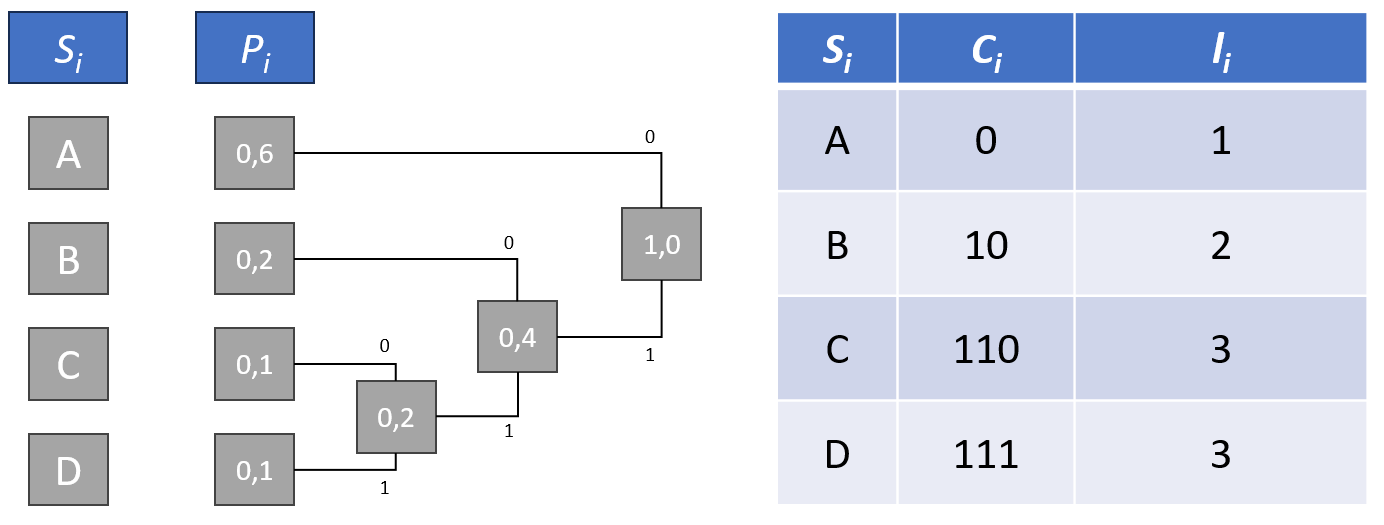
\includegraphics[scale=0.4]{Bilder/Huffmancode_beispiel.png}
  \caption[Huffman Code Beispiel]{\textbf{Erstellen eines Huffman Codes} Die Abbildung zeigt die Konstruktion eins Binärbaums und der daraus resultierenden Codewörter für die Symbole}
  \label{fig:huffman_example}
\end{figure}

Um die mittlere Codewortlänge einer Huffman Codierung zu berechnen, wird die Formel
\begin{equation*}
\bar{l} = \sum_{i=1}^{n} p_i \cdot l_i
\end{equation*}
benötigt \newline

Aus dem Beispiel ergibt sich eine mittlere Codewortlänge von 1,6 \textit{Bits/Symbol} bei einer Huffman Codierung.
Im Vergleich zu einem FLC werden also 0,4 \textit{Bits/Symbol} gespart. \newline

Die Effektivität der Huffman Codierung nimmt ab, je balancierter der konstruierte Binärbaum ist.
Im Umkehrschluss bedeutet das, dass eine Huffman Codierung sehr davon profitiert, dass einzelne Symbole eine höhere Auftrittswahrscheinlichkeit besitzen als die anderen Symbole.
Ändert sich jedoch die Statistik im Laufe der Anwendung, oder wurde diese vorab falsch berechnet, kann eine gute Kompression nicht mehr gewährleistet werden.
Das bedeutet in einem Extremfall, das einem Symbol ein sehr langes Codewort zugeteilt wurde, weil eine sehr geringe Auftrittswahrscheinlichkeit berechnet wurde, die jedoch aus einer kleinen Teilmenge berechnet wurde, und somit nicht repräsentativ für den gesamten Kontext des Eingabestroms ist.

\subsection{GZIP}
\label{subsec:gzip}
Brotli-G misst sich mit anderen Kompressionsstandards wie GZip und Deflate.
Der Deflate Algorithmus beschreibt eine Kombination aus dem LZ77 Algorithmus und der Huffman Codierung

\subsection{Brotli-G Compute Shader}
\label{subsec:brotlig_compute}
Das komprimierte Dreiecksnetz soll mittels Brotli-G's GPU Dekodierer dekodiert werden.
Da Brotli-G mit der Grafik-API DirectX12 arbeitet, wird eine GPU benötigt die das Shader Model 6 unterstützt.
Für die Verwendung des GPU Dekodierers wird also eine NVidia Grafikkarte mit der Turing-Architektur benötigt \cite{Burgess2020}.
Diese erkennt man am RTX Präfix vor der Modellnummer.
Bei AMD Grafikkarten muss mindestens die RDNA-2 Architektur verbaut sein.
Mit Grafikkarten aus der AMD RX6000er Reihe für RDNA-2, und der RX7000er Reihe für RDNA-3 kann der GPU Dekodierer verwendet werden.
Brotli-G definiert ihren GPU Dekodierer in der Shader-Sprache \textit{high-level shader language (HLSL)} und ist als Compute Shader definiert (Kap.~\ref{subsec:compute_shader}).


\subsection{CPU Ebene}
\label{subsec:brotlig_cpu}
Queries Buffers etc
